\documentclass[12pt, a4paper]{article}
% Typography (https://material.io/design/typography/the-type-system.html)

\newcommand{\headlineSix}[1]{
    {\LARGE #1}
}

\newcommand{\subtitleOne}[1]{
    {\Large #1}
}

\newcommand{\subtitleTwo}[1]{
    {\large #1}
}

% Iconography

\newcommand{\icon}[2][20pt]{
    \raisebox{-.25\height}{
        \includesvg[height=#1]{#2}
    }
}

% Table

\newcommand{\rowend}{
    \\[12pt]
}

\newcommand{\lineend}{
    \\[4pt]
}

\newcommand{\tabListItem}[1]{
    \textendash \hspace{4pt} #1
}

% Section

\newcommand{\sectionTitle}[2]{
    \raisebox{-.1\height}{
        \includesvg[height=20pt]{#2}
    }
    \headlineSix{\textbf{#1}}
}

\newcommand{\subsectionTitle}[2]{
    \subtitleOne{#1} \hfill #2
}

\newenvironment{sectionBody}{
    \vspace{-16pt}
    \begin{tabbing}
    \hspace{5mm} \= \\
}
{ 
    \end{tabbing}
    \vspace{-25pt}
}

\newenvironment{subsec}[2]{
    \subsectionTitle{#1}{#2}
    \begin{sectionBody}
}
{
    \end{sectionBody}
}
\newcommand{\kiwiAppUrl}[1]{\href{https://play.google.com/store/apps/details?id=com.skypicker.main}{\underline{\smash{#1}}}}
\newcommand{\kiwiUrl}[1]{\href{https://www.kiwi.com}{\underline{\smash{#1}}}}
\newcommand{\crunchyrollUrl}[1]{\href{https://crunchyroll.com/about/en-gb/index.html}{\underline{\smash{#1}}}}
\newcommand{\vrvAppUrl}[1]{\href{https://https://play.google.com/store/apps/details?id=com.ellation.vrv}{\underline{\smash{#1}}}}
\newcommand{\crunchyrollAppUrl}[1]{\href{https://play.google.com/store/apps/details?id=com.crunchyroll.crunchyroid}{\underline{\smash{#1}}}}
\newcommand{\yopesoUrl}[1]{\href{https://yopeso.com}{\underline{\smash{#1}}}}
\newcommand{\limangoAppUrl}[1]{\href{https://play.google.com/store/apps/details?id=de.limango.shop}{\underline{\smash{#1}}}}
\newcommand{\travodUrl}[1]{\href{https://travod.com}{\underline{\smash{#1}}}}
\newcommand{\aursoftUrl}[1]{\href{https://aursoft.md}{\underline{\smash{#1}}}}

\newcommand{\muniUrl}[1]{\href{https://muni.cz/en}{\underline{\smash{#1}}}}
\newcommand{\muniFiUrl}[1]{\href{https://www.fi.muni.cz}{\underline{\smash{#1}}}}
\newcommand{\muniSsmeFiUrl}[1]{\href{http://ssme.fi.muni.cz/en}{\underline{\smash{#1}}}}
\newcommand{\muniThesis}[1]{\href{https://is.muni.cz/th/zstod/?lang=en}{\underline{\smash{#1}}}}
\newcommand{\usmUrl}[1]{\href{https://usm.md/?lang=en}{\underline{\smash{#1}}}}
\newcommand{\fmiUsmUrl}[1]{\href{http://fmi.usm.md/en}{\underline{\smash{#1}}}}
\newcommand{\infFmiUsmUrl}[1]{\href{http://fmi.usm.md/index.php/en/specialitate-informatica}{\underline{\smash{#1}}}}
\newcommand{\androidCertificationUrl}[1]{\href{https://developers.google.com/certification/associate-android-developer}{\underline{\smash{#1}}}}
\newcommand{\arArticleUrl}[1]{\href{https://code.kiwi.com/forget-the-tape-measure-use-your-phone-instead-5512ad02a3cd}{\underline{\smash{#1}}}}

\newcommand{\linkedinUrl}[1]{\href{https://www.linkedin.com/in/arcadii-rubailo}{\underline{\smash{#1}}}}
\newcommand{\githubUrl}[1]{\href{https://github.com/elderanakain}{\underline{\smash{#1}}}}

% Language
\usepackage[english]{babel}
\usepackage[utf8]{inputenc}
\usepackage{newunicodechar}

% Font
\usepackage[sfdefault]{roboto}

% Page (showframe)
\usepackage[a4paper, total={6in, 8in}, lmargin=0.4cm, rmargin=1cm, tmargin=1cm, bmargin=1cm]{geometry}
\pagenumbering{gobble}
\usepackage[dvipsnames]{xcolor}
\definecolor{primary}{RGB}{156, 204, 101}
\definecolor{light}{RGB}{207, 255, 149}

% Image

\usepackage{graphicx}
\graphicspath{ {images/} }
\usepackage{svg}
\usepackage{float}
\usepackage{tikz}

% Table
\usepackage{array}

\usepackage[hidelinks]{hyperref}

% Metadata
\title{CV}
\author{Arcadii Rubailo}

% Global settings
\setlength{\intextsep}{0pt}
\setlength{\parindent}{0pt}
\setlength{\tabcolsep}{2pt}
\newcommand{\midSectionSpace}{16pt}

% Content
\begin{document}

\begin{tikzpicture}[overlay,remember picture]
    \fill[light, opacity=0.2] (0.31\paperwidth,-\paperheight) rectangle (\paperwidth,\paperheight);
\end{tikzpicture}
\begin{tikzpicture}[overlay,remember picture]
    \fill[primary, opacity=1] (current page.south west) rectangle (0.345\paperwidth,\paperheight);
\end{tikzpicture}
\begin{tikzpicture}[overlay,remember picture]
    \node[inner sep=0pt] at (5pt,-0.75\paperheight) {
\includegraphics[width=0.5\textwidth]{logo_jetpack}};
\end{tikzpicture}
\begin{minipage}[t]{0.35\textwidth}
    \begin{figure}[H]
        \vspace*{-20pt}
        \begin{tikzpicture}
            \clip (0,22pt) circle (90pt); 
            \path (0,0) node{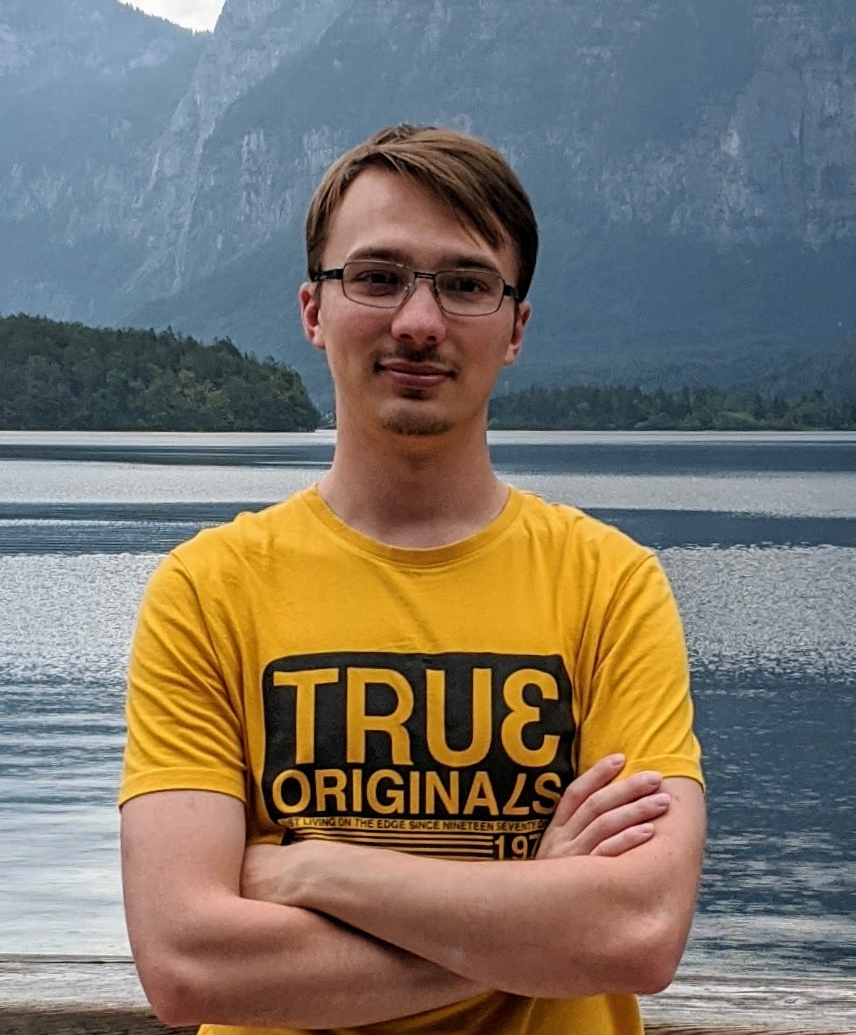
\includegraphics[width=\textwidth]{profile}};
        \end{tikzpicture}
    \end{figure}
   
    \begin{center}
        \headlineSix{\textbf{Arcadii Rubailo}}
        
        \medskip
        
        \subtitleTwo{Android Developer}
    \end{center}
    
    \begin{tabular}{ c l }
        \icon{icon_email}           &   rubailo.arcadii@gmail.com                                               \rowend
        \icon{icon_phone}           &   +420 775 087 503                                                        \rowend
        \icon{icon_home}            &   Videnska 22d, Brno                                                      \\
                                    &   Czech Republic                                                          \rowend
        \icon{icon_flag}            &   Moldova                                                                 \rowend
        \icon[15pt]{icon_linkedin}  &   \linkedinUrl{/arcadii-rubailo}                                          \rowend
        \icon[18pt]{icon_github}    &   \githubUrl{/elderanakain}                                               \rowend
        \icon{icon_language}        &   Russian - Native                                                        \\  
                                    &   English - C1                                                            \\  
                                    &   Romanian - B1                                                           \\  
                                    &   Czech - A1                                                              \rowend
    \end{tabular}
    
    \vspace{255pt}
    
    \repoUrl{written in LaTeX}
\end{minipage}
\hspace{15pt}
\begin{minipage}[t]{0.6\textwidth}
    \sectionTitle{Experience}{icon_work}
    
    \vspace{24pt}
    
    \begin{subsec}{\kiwiUrl{Kiwi.com}}{07.2018 – Present}
        \>  \kiwiAppUrl{Kiwi.com Android application development}.   \lineend
        \>  \tabListItem{ViewModel support for custom views;}        \\
        \>  \tabListItem{\arArticleUrl{AR bag measuring tool};}      \\
        \>  \tabListItem{Booking multi-step architecture;}           \\
        \>  \tabListItem{Mentoring a junior developer.}              \lineend
        \>  Tech stack: Kotlin, Java, MVVM,  Dagger2, Koin, Realm,   \\
        \>  RxJava2, LiveData, Databinding, Jetpack, ARCore, Moshi.  \\
    \end{subsec}
    
    \vspace{\midSectionSpace}
    
    \begin{subsec}{\crunchyrollUrl{Crunchyroll}}{01.2017 – 08.2017}
        \>  \vrvAppUrl{VRV} and \crunchyrollAppUrl{Crunchyroll} Android applications development.   \lineend
        \>  Tech stack: Kotlin, Java, MVP, Dagger2, RxJava2,                                        \\
        \>  Butterknife, Chromecast, Exoplayer.                                                     \\
    \end{subsec}
    
    \vspace{\midSectionSpace}
    
    \begin{subsec}{\yopesoUrl{Yopeso}}{08.2016 – 01.2017}
        \>  \limangoAppUrl{limango} Android application development.    \lineend
        \>  Tech stack: Java, MVP, Dagger2, RxJava, SQLite.             \\
    \end{subsec}

    \vspace{\midSectionSpace}
    
    \begin{subsec}{\travodUrl{Travod}}{10.2015 – 08.2016}
        \>  Translation and localisation services.  \\
        \>  \tabListItem{Project management;}       \\
        \>  \tabListItem{Technical support.}        \\
    \end{subsec}

    \vspace{\midSectionSpace}
    
    \begin{subsec}{\aursoftUrl{Aursoft}}{02.2015 – 12.2015}
        \> MyBebe Android application development. \lineend
        \> Tech stack: Java, Volley, Picasso, SQLite. \\
    \end{subsec}
    
    \vspace{24pt}
    
    \sectionTitle{Education}{icon_school}
    
    \vspace{24pt}
    
    \begin{subsec}{Android certification}{2020}
        \> \androidCertificationUrl{Google Associate Android Developer Certification} \\
    \end{subsec}
    
    \vspace{\midSectionSpace}
    
    \begin{subsec}{\muniUrl{Masaryk University}}{2017 – 2019}
        \> Master of Science, \muniFiUrl{Faculty of Informatics} \\
        \> Service Science, Management and Engineering \\
        \> \muniThesis{Thesis} \\
    \end{subsec}
    
    \vspace{\midSectionSpace}
    
    \begin{subsec}{\usmUrl{State University of Moldova}}{2014 – 2017}
        \> Bachelor of Science, \fmiUsmUrl{Mathematics and Computer Science} \\
        \> Computer science \\
    \end{subsec}
\end{minipage}
\end{document}
